\chapter{Implementation using FEniCS and Firedrake}

In this appendix, some tools needed for low-level manipulation of the \fenics and \firedrake libraries are illustrated. It is assumed to a recent version of \fenics and \firedrake is available, either through local installation (Anaconda or installation from source for \fenics and virtual Python environment for \firedrake) or through Docker containers. Additional information concerning the installation can be found at \url{https://fenicsproject.org/download/} for \fenics and \url{https://www.firedrakeproject.org/download.html} for \firedrake. The \fenics library possesses a vast documentation \cite{logg2012}. On the contrary, the \firedrake developers have not released a comprehensive book, and employ tutorials to illustrate the functioning of the library. Boxes colored in red are used for \textcolor{red}{\fenics}, cyan for \textcolor{cyan}{\firedrake} and gray for identical commands in both libraries. The libraries are assumed to be loaded through the star import:	
\begin{verbatim}
from fenics import *
\end{verbatim}
or
\begin{verbatim}
from firedrake import *
\end{verbatim}
\paragraph{Creation of a mixed function space}
For the discretization of pHs one has to use a mixed function space, i.e. a collection of more than one function space. Consider the creation of the Mindlin plate CGDG elements \eqref{eq:CGDG} on a unit square simplicial mesh with 40 elements per side.
\begin{tcolorbox}[title = Mixed function space in  \fenics, coltitle=black, breakable, size=fbox, boxrule=1pt, pad at break*=1mm, colframe=red, enlarge top by=0.25em, enlarge bottom by=0.5em]
\begin{Verbatim}[tabsize=4]
n_el  = 40
mesh  = UnitSquareMesh(n_el, n_el)
P_w   = FiniteElement('CG', triangle, 1)   	% vertical velocity
P_th  = VectorElement('CG', triangle, 1)   	% angular velocity
P_kap = VectorElement('DG', triangle, 0, dim=3)	% bending momenta			
P_gam = VectorElement('DG', triangle, 0)	% shear stress 
elem  = MixedElement([P_pw, P_pth, P_qth, P_qw])
V     = FunctionSpace(mesh, elem)
\end{Verbatim}
\end{tcolorbox}
\begin{tcolorbox}[title = Mixed function space in  \firedrake, coltitle=black, breakable, size=fbox, boxrule=1pt, pad at break*=1mm, colframe=cyan, enlarge top by=0.25em, enlarge bottom by=0.5em]
\begin{Verbatim}[tabsize=4]
n_el  = 40
mesh  = UnitSquareMesh(n_el, n_el)
V_w   = FunctionSpace(mesh, "CG", 1)
V_th  = VectorFunctionSpace(mesh, "CG", 1)
V_kap = VectorFunctionSpace(mesh, "DG", 0, dim=3)
V_gam = VectorFunctionSpace(mesh, "DG", 0)
V     = MixedFunctionSpace([V_w, V_th, V_kap, V_gam])
\end{Verbatim}
\end{tcolorbox}
The space $\verb|V_kap|$ has dimension 3 since it corresponds to variable $\bm{E}_\kappa \in \bbR^{2\times 2}_{\text{sym}} \cong  \bbR^3$.

\paragraph{Definition of a variational form}
The precedent commands create a function space that can be used to construct variational forms trough the Unified Form Language \cite{alnaes2014} (UFL). UFL is a core component of \fenics and has been adopted in \firedrake as well. It is an expressive domain-specific language for abstractly representing (finite element) variational formulations of differential equations. In particular, this language defines a syntax for the integration of variational forms over various domains. This simply leads to an expressive implementation that is close to the abstract mathematical formulations. Given the previously defined function space, consider the definition of variational forms representing the mass matrix $\mathbf{M}$ and interconnection matrix $\mathbf{J}$ (the implementation is the same in both libraries).
 
\begin{tcolorbox}[title = Definition of the variational form (\fenics \& \firedrake), coltitle=white, breakable, size=fbox, boxrule=1pt, pad at break*=1mm, enlarge top by=0.25em, enlarge bottom by=0.5em]
\begin{Verbatim}[tabsize=4]
% Physical parameters 
E   = 1e12
nu  = 0.3	
rho = 2600
h   = 0.1
k   = 5/6	
G   = E / 2 / (1 + nu)
F   = G * h * k

% Definition of the bending curvature operator
def bending_curv(mom):
	kappa = 12. / (E * h ** 3) * ((1+nu)*mom - nu * Identity(2) * tr(mom))
	return kappa
	
% Test variables
v = TestFunction(V)
v_w, v_th, v_kap, v_gam = split(v)	

% Co-energy variables
e = TrialFunction(V)
e_w, e_th, e_kap, e_gam = split(e)

% Convert the R^3 vector to a symmetric tensor
v_kap = as_tensor([[v_kap[0], v_kap[1]],
				   [v_kap[1], v_kap[2]]])
e_kap = as_tensor([[e_kap[0], e_kap[1]],
				   [e_kap[1], e_kap[2]]])
			
% Energy variables   
a_w   = rho * h * e_w
a_th  = (rho * h ** 3) / 12. * e_th
a_kap = bending_curv(e_kap)
a_gam = 1. / F * e_gam

% Mass bilinear form 
m_form = v_w * a_w * dx + dot(v_th, a_th) * dx + \
		 inner(v_kap, a_kap) * dx + dot(v_gam, a_gam) * dx 

% Interconnection bilinear form
j_form = dot(v_gam, grad(e_w)) * dx - dot(grad(v_w), e_gam) * dx + \
		 inner(v_kap, sym(grad(e_th))) * dx - \
		 inner(sym(grad(v_th)), e_kap) * dx + \
		 dot(v_th, e_gam) * dx - dot(v_gam, e_th) * dx
\end{Verbatim}
\end{tcolorbox}

\paragraph{Matrices assemble}
Once the forms have been declared, it is possible to actually construct the associated matrices. Consider the case of a clamped (i.e. Dirichlet) boundary condition. For the CGDG elements a clamped condition corresponds to essential boundary conditions. These are defined in the same way in \fenics and \firedrake
\begin{tcolorbox}[title = Dirichlet boundary conditions, coltitle=white, breakable, size=fbox, boxrule=1pt, pad at break*=1mm, enlarge top by=0.25em, enlarge bottom by=0.5em]
\begin{Verbatim}[tabsize=4]
bcs = []
bcs.append(DirichletBC(V.sub(0), Constant(0.0), "on_boundary"))
bcs.append(DirichletBC(V.sub(1), Constant((0.0, 0.0)), "on_boundary"))
\end{Verbatim}
\end{tcolorbox}
The subspaces \verb|V.sub(0)|, \verb|V.sub(1)| correspond to spaces \verb|V_w|, \verb|V_th| associated to the vertical velocity and the angular velocity, respectively. The boundary conditions can now be incorporated in the matrices. The final assemble of the matrices is achieved in \fenics by the following code snippet.
\begin{tcolorbox}[title = Matrices assembly in  \fenics, coltitle=black, breakable, size=fbox, boxrule=1pt, pad at break*=1mm, colframe=red, enlarge top by=0.25em, enlarge bottom by=0.5em]
	\begin{Verbatim}[tabsize=4]
	J, M = PETScMatrix(), PETScMatrix()
	dummy = v_pw * dx
	assemble_system(j_form, dummy, bcs, A_tensor=J)
	assemble_system(m_form, dummy, bcs, A_tensor=M)
	\end{Verbatim}
\end{tcolorbox}
Matrices are first defined as {\sc{PETSc}} matrices and forms are assembled into it. The boundary conditions have been applied to the stiffness matrix using \verb|assemble_system| so as to preserve symmetry (a dummy right-hand side vector have been introduced to call this function). The same matrices are constructed in \firedrake by the following code
\begin{tcolorbox}[title = Matrices assembly in  \firedrake, coltitle=black, breakable, size=fbox, boxrule=1pt, pad at break*=1mm, colframe=cyan, enlarge top by=0.25em, enlarge bottom by=0.5em]
	\begin{Verbatim}[tabsize=4]
	J = assemble(j_form, bcs=bcs, mat_type='aij')
	M = assemble(m_form, bcs=bcs, mat_type='aij')
	petsc_j = J.M.handle
	petsc_m = M.M.handle
	\end{Verbatim}
\end{tcolorbox}
The option \verb|mat_type| specifies the desired format for the matrix representation. To get a final {\sc{PETSc}} matrix, the AIJ format is used. The methods \verb|J.M.handle|, \verb|M.M.handle| provide as outputs $\verb|J|, \; \verb|M|$ that are {\sc{PETSc}} matrices. These can be manipulated using the \verb|petsc4py| library\footnote{\url{https://www.mcs.anl.gov/petsc/petsc4py-current/docs/apiref/index.html}}. For what concerns the ordering of the degrees of freedom, \firedrake just piles up the degrees of freedom of each subspace. The final matrices have the same structure as in \eqref{eq:pHfindim_Min_grad}. For \fenics the default option is a not-natural ordering to cluster the non-zero entries closer to the diagonal. A natural ordering can be set by changing the \verb|reorder_dofs_serial| parameters\footnote{\url{https://fenicsproject.discourse.group/t/ordering-of-mixed-elements/946}}.

\paragraph{Eigenvalues computation}
A simple test to assess the validity of the finite element discretization consists in computing the eigenvalues of the matrices, to assess the absence of spurious modes. The {\sc{SLEPc}} library is used to this end \footnote{\url{https://slepc.upv.es/documentation/slepc.pdf}} \cite{hernandez2005slepc}. Since we are interested in the lowest eigenvalues, a shift-and-invert method is used. The following code compute the eigenvalues.
\begin{tcolorbox}[title = Eigenvalues computation in  \fenics, coltitle=black, breakable, size=fbox, boxrule=1pt, pad at break*=1mm, colframe=red, enlarge top by=0.25em, enlarge bottom by=0.5em]
\begin{Verbatim}[tabsize=4]
solver = SLEPcEigenSolver(J, M)
solver.parameters["solver"] = "krylov-schur"
solver.parameters["problem_type"] = "pos_gen_non_hermitian"
solver.parameters["spectrum"] = "target imaginary"
solver.parameters["spectral_transform"] = "shift-and-invert"
solver.parameters["spectral_shift"] = 1/((2*(1+nu)*rho)/E)**0.5
solver.solve(40)
nconv = solver.get_number_converged()
for i in range(nconv):
	r, c, rx, cx = solver.get_eigenpair(i)
\end{Verbatim}
\end{tcolorbox}
The shift is given to make the eigensolver look for the first eigenvalue. For \firedrake the equivalent code snippet is the following.
\begin{tcolorbox}[title = Eigenvalues computation in  \firedrake, coltitle=black, breakable, size=fbox, boxrule=1pt, pad at break*=1mm, colframe=cyan, enlarge top by=0.25em, enlarge bottom by=0.5em]
\begin{Verbatim}[tabsize=4]
from firedrake.petsc import PETSc
try:
	from slepc4py import SLEPc
except ImportError:
	import sys
	warning("Unable to import SLEPc (try firedrake-update --slepc)")
	sys.exit(0)

opts = PETSc.Options()
opts.setValue("pos_gen_non_hermitian", None)
opts.setValue("st_pc_factor_shift_type", "NONZERO")
opts.setValue("eps_type", "krylovschur")
opts.setValue("eps_tol", 1e-10)
opts.setValue("st_type", "sinvert")
opts.setValue("st_shift", 1/(((2*(1+nu)*rho)/E)**0.5))
opts.setValue("eps_target", 1/(((2*(1+nu)*rho)/E)**0.5))

es = SLEPc.EPS().create(comm=COMM_WORLD)
es.setDimensions(40)
es.setOperators(petsc_j, petsc_m)
es.setFromOptions()
es.solve()

nconv = es.getConverged()
vr, vi = petsc_j.getVecs()
for i in range(nconv):
	lam = es.getEigenpair(i, vr, vi)
\end{Verbatim}
\end{tcolorbox}


\begin{figure*}[tb]
	\centering
	\subfloat[$\widehat{\omega}_1 = 1.60$]{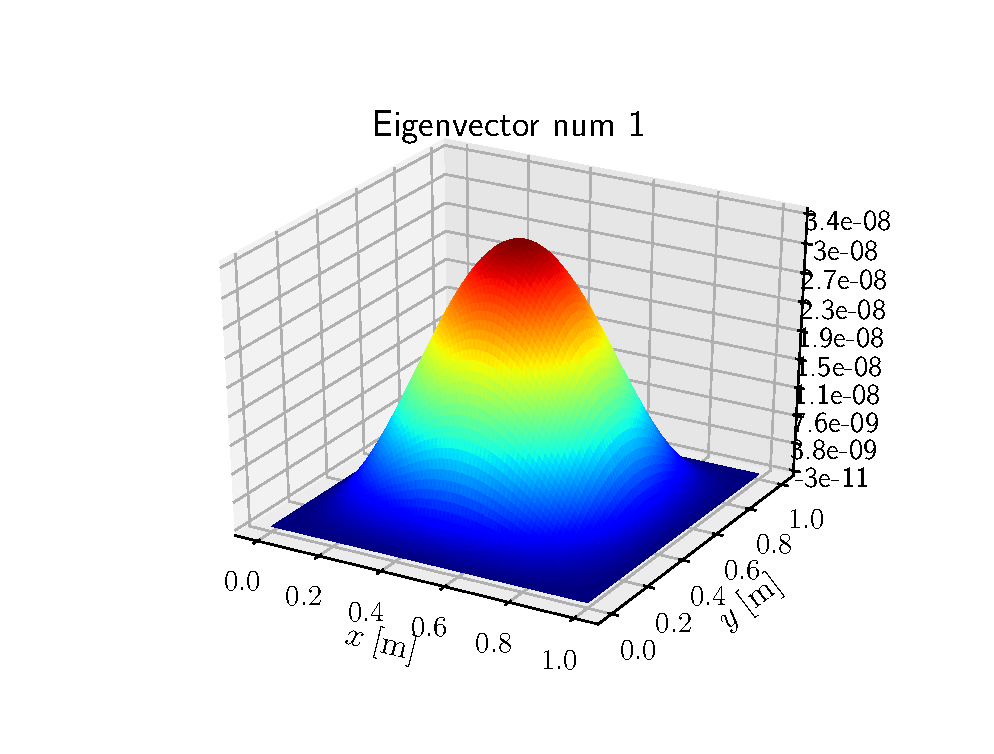
\includegraphics[width=0.5\linewidth]{appendix/Eig1.eps}%
		\label{fig:Eig1}}
	\hfil
	\subfloat[$\widehat{\omega}_2 = 3.06$]{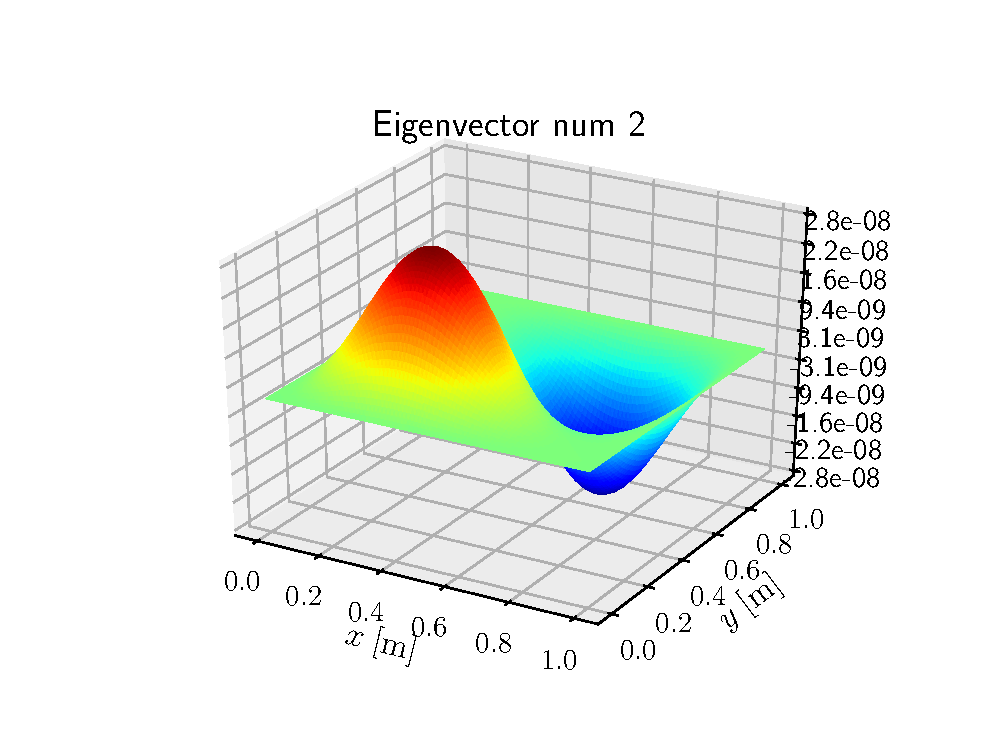
\includegraphics[width=0.5\linewidth]{appendix/Eig2.eps}%
		\label{fig:Eig2}} \\
	\subfloat[$\widehat{\omega}_3 = 3.07$]{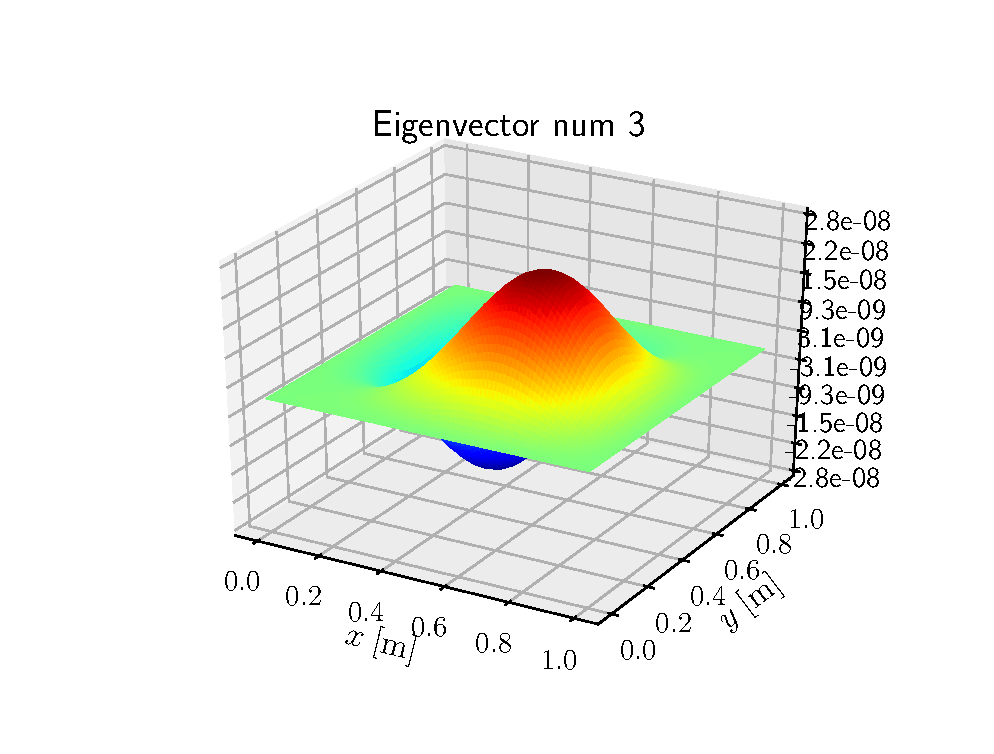
\includegraphics[width=0.5\linewidth]{appendix/Eig3.eps}%
		\label{fig:Eig3}}
	\hfil
	\subfloat[$\widehat{\omega}_4 = 4.31$]{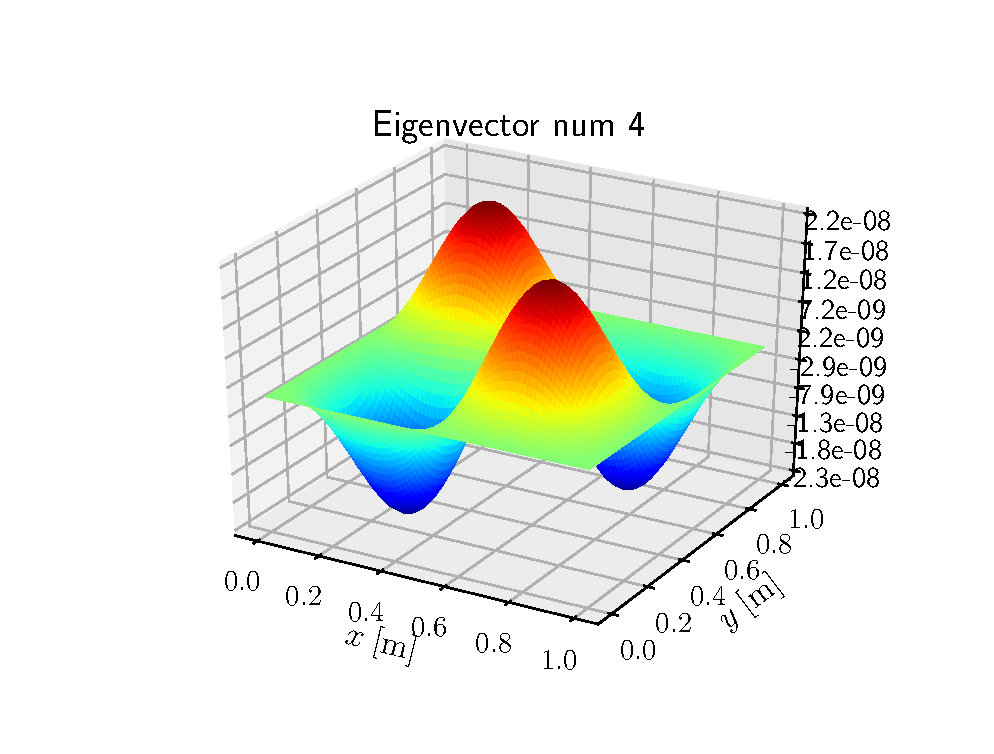
\includegraphics[width=0.5\linewidth]{appendix/Eig4.eps}%
		\label{fig:Eig4}}
	\caption{Eigenvectors for the clamped Mindlin plate computed with \firedrake. The eigenfrequencies are normalized $\widetilde{\omega} = \omega((2(1+\nu)\rho/E)^{1/2}$. The results are consistent with \cite{duran1999approximation}.}
	\label{fig:EigMin}
\end{figure*}

\paragraph{Conversion to \textsc{Scipy} for direct manipulation of the boundary matrices}
If boundary control has to be taken into account, it is preferable to move to \textsc{Scipy} for the implementation. Consider now the case of a Mindlin plate with Neumann boundary control. The construction of the mass and interconnection matrices is the same, without imposing any boundary conditions.

\begin{tcolorbox}[title = Eigenvalues computation in  \firedrake, coltitle=black, breakable, size=fbox, boxrule=1pt, pad at break*=1mm, colframe=cyan, enlarge top by=0.25em, enlarge bottom by=0.5em]
\begin{Verbatim}[tabsize=4]
n = FacetNormal(mesh)

V_qn = FunctionSpace(mesh, 'Lagrange', 1)
V_Mnn = FunctionSpace(mesh, 'Lagrange', 1)

Vu = V_qn * V_Mnn

q_n, M_nn = TrialFunction(Vu)

v_omn = dot(grad(v_p), n)
g_vec = []
for key, val in bc_dict.items():
if val == 'C':
g_vec.append(v_p * q_n * ds(key) + v_omn * M_nn * ds(key))
elif val == 'S':
g_vec.append(v_p * q_n * ds(key))

g_lmb = sum(g_vec)
\end{Verbatim}
\end{tcolorbox}


